\documentclass{article}

\usepackage{graphicx} % Required for inserting images
\usepackage{amsmath}
\usepackage{hyperref}

\usepackage[utf8]{inputenc} 
\usepackage[ngerman]{babel} 
\usepackage[T1]{fontenc}   

\title{Mein erstes LaTeX Dokument}
\author{Lennart Oelschläger}
\date{15.10.2024}

\begin{document}

% Title, Autor und Datum erzeugen
\maketitle

% Abstract
\begin{abstract}
    Dies ist ein einfacher Absatz am Anfang des Dokuments. Eine kurze Einführung in das Hauptthema.
\end{abstract}

% Inhaltsverzeichnis
\tableofcontents

% starte mit dem Inhalt auf der nächsten Seite
\newpage

\section{Mathematische Formeln}

\begin{enumerate}
    \item Formeln können so $f(x) = x^2$ eingegeben werden. 
    \item Umfangreichere Formeln können wir absetzen:
    $$ \exp(x) =  \lim_{n \to \infty} \left( 1 + \frac{1}{n} \right)^n $$
    \item Wir können solche Formeln auch nummerieren ...
    \begin{equation}
        \label{eq:exponential_function}
        \exp(x) = \sum_{n = 0}^\infty \frac{x^n}{n!}
    \end{equation}
    ... und später diese Formel mit \eqref{eq:exponential_function} referenzieren.
\end{enumerate}

\section{Auflistungen}

\subsection{Variante 1}

% Textformatierung
Die \textbf{jährlichen} \underline{Benzinkosten $C$} ergeben sich aus dem \textit{Produkt} des Preises $P$ pro Liter Benzin, der Benzinverbrauch $V$ in Liter pro Kilometer und der Kilometeranzahl $K$ pro Jahr.

\subsection{Variante 2}

Die jährlichen Benzinkosten ergeben sich aus $$ C = P \cdot L \cdot K, $$ wobei

\begin{itemize}
    \item $C$ die jährlichen Benzinkosten,
    \item $P$ den Preis pro Liter Benzin,
    \item $V$ den Benzinverbrauch in Liter pro Kilometer und
    \item $K$ die Kilometerzahl pro Jahr bezeichnet.
\end{itemize}

\section{Grafiken}

Grafiken können mit der \texttt{figure}-Umgebung beschriftet und referenziert werden:

\begin{figure}[h] % oder t, falls Grafiken immer oben ("top") erscheinen sollen
    \centering
    % benötigt \usepackage{graphicx} in der Präambel
    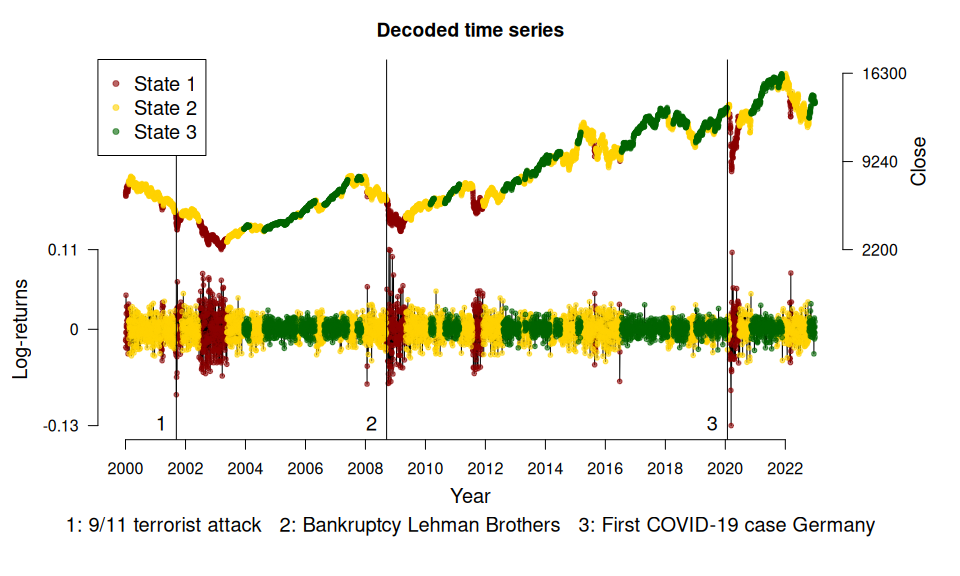
\includegraphics[width = \textwidth]{time_series.png}
    % mit in \renewcommand{\figurename}{Abbildung} zu "Abbildung" umbenennen
    \caption{Der Verlauf des DAX}
    \label{fig:dax}
\end{figure}

Abbildung \ref{fig:dax} zeigt den Verlauf des Deutschen Aktienindex (DAX). Er wurde mithilfe eines Hidden Markov Models (HHM) dekodiert.

\section{Absätze}

Wir können den ersten Absatz beginnen und dann zweimal die ``Enter''-Taste drücken, um den zweiten zu starten.

Diese Zeile beginnt einen zweiten Absatz.

Ich werde den dritten Absatz beginnen und dann einen \\ manuellen Zeilenumbruch hinzufügen, wodurch dieser Text auf einer neuen Zeile beginnt, aber Teil desselben Absatzes bleibt.

Es wird empfohlen, mehrere \verb|\\| nicht zu verwenden, um ``größere Abstände'' zwischen Absätzen zu simulieren. Die empfohlene Methode ist, weiterhin leere Zeilen für neue Absätze zu verwenden, und das Paket \texttt{parskip} in der Präambel zu laden.

\end{document}